%% LyX 2.3.2 created this file.  For more info, see http://www.lyx.org/.
%% Do not edit unless you really know what you are doing.
\documentclass{beamer}
\usepackage[T1]{fontenc}
\usepackage[utf8]{inputenc}
\usepackage[czech]{babel}
\babelprovide[import,main]{czech}
\usepackage{textcomp}
\usepackage{url}
\usepackage{lmodern}
\usepackage{amsmath}
\usepackage{amssymb}
\usepackage{graphicx}
\usepackage{makecell}
\usepackage{wrapfig}
\usepackage{wasysym}
\usepackage{listings}

\usepackage{enumitem}
\setlistdepth{9}
\setlist[itemize,1]{label=$\bullet$}
\setlist[itemize,2]{label=$\bullet$}
\setlist[itemize,3]{label=$\bullet$}
\setlist[itemize,4]{label=$\bullet$}
\setlist[itemize,5]{label=$\bullet$}
\setlist[itemize,6]{label=$\bullet$}
\setlist[itemize,7]{label=$\bullet$}
\setlist[itemize,8]{label=$\bullet$}
\setlist[itemize,9]{label=$\bullet$}

\renewlist{itemize}{itemize}{9}

\usepackage[export]{adjustbox}
\ifx\hypersetup\undefined
  \AtBeginDocument{%
    \hypersetup{unicode=true}
  }
\else
  \hypersetup{unicode=true}
\fi

\makeatletter

%%%%%%%%%%%%%%%%%%%%%%%%%%%%%% LyX specific LaTeX commands.
%% Because html converters don't know tabularnewline
\providecommand{\tabularnewline}{\\}

%%%%%%%%%%%%%%%%%%%%%%%%%%%%%% Textclass specific LaTeX commands.
% this default might be overridden by plain title style
\newcommand\makebeamertitle{\frame{\maketitle}}%
% (ERT) argument for the TOC
\AtBeginDocument{%
  \let\origtableofcontents=\tableofcontents
  \def\tableofcontents{\@ifnextchar[{\origtableofcontents}{\gobbletableofcontents}}
  \def\gobbletableofcontents#1{\origtableofcontents}
}

%%%%%%%%%%%%%%%%%%%%%%%%%%%%%% User specified LaTeX commands.
\usepackage{listings}
\usetheme{Warsaw}
% or ...
%\usetheme{Antibes}	% tree outline, neat
%\usetheme{JuanLesPins}	% like Antibes, with shading
%\usetheme{Bergen}	% outline on side
%\usetheme{Luebeck}	% like Warsaw, square sides
%\usetheme{Berkeley}	% interesting left bar outline
%\usetheme{Madrid}	% clean, nice.  7/12 page numbers
%\usetheme{Berlin}	% dots show slide number
%\usetheme{Malmoe}	% OK, plain, unshaded
%\usetheme{Boadilla}	% nice, white bg, no top bar
%\usetheme{Marburg}	% nice, outline on right
%\usetheme{boxes}	% ???
%\usetheme{Montpellier}	% tree outline on top, plainish white
%\usetheme{Copenhagen}	% like Warsaw
%\usetheme{PaloAlto}	% looks good
%\usetheme{Darmstadt}	% like Warsaw with circle outline
%\usetheme{Pittsburgh}
%\usetheme{default}
%\usetheme{Rochester}	% like boxy, unshaded warsaw
%\usetheme{Dresden}	% circle outline on top
%\usetheme{Singapore}	% purple gradient top
%\usetheme{Frankfurt}	% like Warsaw with circle outline on top
%\usetheme{Szeged}
%\usetheme{Goettingen}	% light purple right bar outline
%\usetheme{Warsaw}
%\usetheme{Hannover}	% like Goett with bar on left
%\usetheme{compatibility}
%\usetheme{Ilmenau}

\setbeamercovered{transparent}
% or whatever (possibly just delete it)

%\usecolortheme{seahorse}
%\usecolortheme{rose}

% seems to fix typewriter font in outline header:
\usepackage{ae,aecompl}

\newcommand{\putat}[3]{\begin{picture}(0,0)(0,0)\put(#1,#2){#3}\end{picture}}

\makeatother

\begin{document}
\title[Aktualizace embedded systém\r{u} pomocí NuttX bootloaderu]{Aktualizace embedded systém\r{u} pomocí NuttX bootloaderu}

\author[CC-BY 2025: Michal Lenc]{Michal Lenc, Pavel Pí\v{s}a, Karel Ko\v{c}í, \v{S}t\v{e}pán Pressl\\\small{michallenc@seznam.cz}}
\institute[shortinst]{Elektroline a.s, ČVUT FEL}

%\affiliation{La Scuola universitaria professionale della Svizzera italiana, Department of Innovative Technologies}{SUPSI}

\date{2025-03-16\\InstallFest 2025}

\makebeamertitle

\AtBeginSection[]{
  \frame<beamer>{
    \frametitle{Outline}
    \tableofcontents[currentsection,currentsubsection]
  }
}

%\beamerdefaultoverlayspecification{<+->}
%\begin{frame}{Content of Presentation}

%{\small{}\tableofcontents{}}{\small\par}
%\end{frame}

\begin{frame}{Use-case a požadavky}
  \begin{itemize}
    \item embedded zařízení v rozvaděčích, tramvajích...
    \item připojení typicky přes CAN
    \item relativně velký image (vyšší stovky kB)
    \item možnost externí NOR paměti, update image nahráván do ní
    \item potřebné vlastnosti:
    \begin{itemize}
      \item vzdálená aktualizace firmwaru (over-the-air)
      \item nahrávání nového firmwaru za běhu původní aplikace (A/B update)
      \item update provedený po restarování zařízení nakopírováním do programové flash paměti
      \item explicitní potvrzení nového firmwaru
      \item vrácení původního firmwaru v případě nepotvrzení/chyby
      \item krátký čas aktualizace (bez zápisu na NOR)
    \end{itemize}
    \item možná integrace s NuttX OS
  \end{itemize}
\end{frame}

\begin{frame}{NuttX}
  \begin{itemize}
    \item otevřený RTOS, Apache License 2.0
    \begin{itemize}
      \item \url{https://nuttx.apache.org/}
    \end{itemize}
    \item kompatibilní s POSIX standardem
    \item široká podpora architektur (ARM, AVR, RISC-V...) a desek
  \end{itemize}
  \begin{columns}
    \begin{column}{0.70\textwidth}
      \begin{itemize}
        \item psán v C, Kconfig syntaxe (Linux)
        \item publikován v roce 2007, relativně mature
        \item před několika lety pro něj přidána podpora do MCUboot projektu
        \vfil
      \end{itemize}
    \end{column}
    \begin{column}{0.2\textwidth}
      \begin{center}
        \includegraphics[width=1\textwidth]{figs/nuttx}
      \par\end{center}
      \vfil
    \end{column}
  \end{columns}
\end{frame}

\begin{frame}{MCUboot}
  \begin{itemize}
    \item otevřený secure bootloader
    \begin{itemize}
      \item \url{https://docs.mcuboot.com/}
    \end{itemize}
    \item hodně využívaný se Zephyrem, ale podporuje též NuttX
    \item o nahrání nového firmwaru se stará aplikace, ne bootloader
    \item mechanismus potvrzení a případného revertu
    \item spousta operačních módů (XIP, RAM load, copy only)
    \item pro nás zajímavé swap algoritmy
    \begin{itemize}
      \item swap using scratch
      \item swap using offset
      \item swap using move
    \end{itemize}
  \end{itemize}
\end{frame}

\begin{frame}{Swap algoritmy}
  \begin{itemize}
    \item využívají dva oddíly (primary, secondary)
    \item update nahrán do secondary a po rebootu překlopen do primary
    \item primary se zároveň překlopí do secondary a slouží jako záloha
    \item scratch algoritmus má ještě třetí oddíl, který slouží jako odkladiště části kopírovaného firmwaru 
    \item offset a move mají secondary o něco větší a toto odkladiště posouvají v ní
    \item nevýhody a problémy
    \begin{itemize}
      \item scratch likvidována častým mazáním
      \item nutnost vytvoření zálohy při každém updatu, výrazný bottleneck pokud je secondary v externí paměti
      \item postup updatu držen v ocásku, image pro MCUboot má padding na velikost oddílu
      \item potvrzení provádí aplikace zápisem do paměti, ze které běží (flag v tailu)
    \end{itemize}
  \end{itemize}
\end{frame}

\begin{frame}{Jak to vyřešit?}
  \begin{itemize}
    \item potřeba eliminovat zápis na NOR -> záloha by měla být dostupná pořád a nevytvářet se během updatu
    \item to se 2 oddíly nejde, jsou potřeba tři
    \item větší nároky na paměť, ale rychlejší update
  \end{itemize}
  \begin{center}
    \includegraphics[width=1\textwidth]{figs/01}
  \end{center}
\end{frame}

\begin{frame}{Jak to vyřešit?}
  \begin{center}
    
\includegraphics[width=1.1\textwidth, center]{figs/02}
  \par\end{center}
\end{frame}

\begin{frame}{Jak to vyřešit?}
  \begin{center}
    \includegraphics[width=1.1\textwidth, center]{figs/03}
  \par\end{center}
\end{frame}

\begin{frame}{Jak to vyřešit?}
  \begin{center}
    \includegraphics[width=1.1\textwidth, center]{figs/04}
  \par\end{center}
\end{frame}

\begin{frame}{Jak to vyřešit?}
  \begin{center}
    
\includegraphics[width=1.1\textwidth, center]{figs/05}
  \par\end{center}
\end{frame}

\begin{frame}{Jak to vyřešit?}
  \begin{center}
    \includegraphics[width=1.1\textwidth, center]{figs/06}
  \par\end{center}
\end{frame}

\begin{frame}{Jak to vyřešit?}
  \begin{itemize}
    \item záloha je vlastně již zapsaná aplikací při nahrání aktualizace
    \begin{itemize}
      \item výjimkou je první update, kdy je potřeba udělat zálohu z primary
    \end{itemize}
    \item méně mazání -> šetrnější na paměť
    \item první update trvá déle, další již jen zapisují do programové paměti
    \item zkrácena doba updatu z cca 4-5 minut na 20 sekund (pro 2 MB image)
    \item pořád některé nevýhody
    \begin{itemize}
      \item image má padding na velikost oddílu kvůli tailu
      \item potvrzení prováděno zápisem do programové paměti
      \item potřeba 3 oddíly, větší nároky na paměť
    \end{itemize}
    \item merge request nového algoritmu do MCUboot odmítnut \frownie
  \end{itemize}
\end{frame}

\begin{frame}{Jak vlastně vypadá implementace bootloaderu}
  Pokud vynecháme šifrování a podpisy, tak relativně jednoduše
  \begin{itemize}
    \item v primární paměti na začátku bootloader, s nějakým offsetem image
    \item image má hlavičku, případně ocásek
    \item bootloader podle hlavičky/ocásku rozhoduje operaci
    \item náš algoritmus vlastně jen kopíruje image mezi oddíly
    \item dvě vrstvy
    \begin{itemize}
      \item algoritmická/rozhodovací
      \item přístup k oddílům přes MTD vrstvu
    \end{itemize}
  \end{itemize}
  Proč si tedy nezkusit napsat vlastní bootloader přímo do NuttXu?
\end{frame}

\begin{frame}{NXBoot design -- hlavička}
  \begin{itemize}
    \item magic -- speciální hodnota určující, že jde o image k bootloaderu
    \item verze hlavičky -- kvůli kompatabilitě změn
    \item velikost hlavičky -- za hlavičkou začíná image
    \item crc -- vypočteno ze zbytku hlavičky a image
    \item velikost image
    \item identifikátor -- unikátní číslo, image odmítnut, pokud jeho identifikátor neodpovídá uloženému v bootloaderu
    \item adresa další hlavičky -- pro budoucí rozšíření
    \item verze image -- podle Semantic Versioning 2.0 (bez metadat)
  \end{itemize}
\end{frame}

\begin{frame}[fragile]{NXBoot design -- hlavička}
  \begin{verbatim}
    struct nxboot_img_header
    {
      uint32_t magic;
      struct nxboot_hdr_version hdr_version;
      uint16_t header_size;
      uint32_t crc;
      uint32_t size;
      uint64_t identifier;
      uint32_t extd_hdr_ptr;
      struct nxboot_img_version img_version;
    };
  \end{verbatim}
  Verze image podle Semantic Versioning 2.0 (bez metadat)
\end{frame}

\begin{frame}{NXBoot design -- ocásek}
  \begin{itemize}
    \item normálně obsahuje informace o potvrzení, případně další metadata
    \item v případě našeho algoritmu je potřeba i označit image jako již nahraný do primary
    \item je ale vůbec potřeba?
    \begin{itemize}
      \item zneplatnění image po nahrání do primary provedeme smazáním první erase page
      \item při potvrzení primary se pak tato erase page zapíše zpátky
      \item tím i máme potvzení -> pokud má image v B/C zálohu, pak je potvrzen
    \end{itemize}
    \item je to ideální?
    \begin{itemize}
      \item první sektor v B/C dvakrát více namáhán, ale zase se střídají
      \item potvrzení může trvat déle, zapisuje se celá erase page (po write pagích)
    \end{itemize}
  \end{itemize}
  Problém s imagem nahraným přes programátor, byl by nestabilní...
\end{frame}

\begin{frame}{NXBoot design}
  \begin{itemize}
    \item řešením další interní magic
    \item při aktualizaci se do primárního oddílu zapíše tento interní magic
    \item klasický magic tak bude nahráván jen přes programátor -> vždy stabilní
    \item B/C oddíly naopak -> klasický update, interní záloha
    \item první dva bity interního vyhrazeny jako pointer na zálohu
    \begin{itemize}
      \item potřeba pro určení správného update slotu po smazání první erase page
      \item zároveň trochu zjednoduší interní logiku
    \end{itemize}
  \end{itemize}
\end{frame}

\begin{frame}{NXBoot design -- úvodní stav}
  \begin{center}
    \includegraphics[width=1.1\textwidth, center]{figs/07}
  \par\end{center}
  \begin{itemize}
    \item v A nahraný image s normálním magic -> potvrzený
    \item B/C prázdné
  \end{itemize}
\end{frame}

\begin{frame}{NXBoot design -- nahrání updatu}
  \begin{center}
    \includegraphics[width=1.1\textwidth, center]{figs/08}
  \par\end{center}
  \begin{itemize}
    \item v A nahraný image s normálním magic -> potvrzený
    \item do B nahrán image s normálním magic -> update
  \end{itemize}
\end{frame}

\begin{frame}{NXBoot design -- vytvoření zálohy}
  \begin{center}
    \includegraphics[width=1.1\textwidth, center]{figs/09}
  \par\end{center}
  \begin{itemize}
    \item po rebootu se do C uloží záloha s interním magic
    \item update začne po skončení zálohy
  \end{itemize}
\end{frame}

\begin{frame}{NXBoot design -- aktualizace}
  \begin{center}
    \includegraphics[width=1.1\textwidth, center]{figs/10}
  \par\end{center}
  \begin{itemize}
    \item z B se do A nakopíruje nový image
    \item je potřeba zneplatnit B
  \end{itemize}
\end{frame}

\begin{frame}{NXBoot design -- zneplatnění hlavičky aktualizace}
  \begin{center}
    \includegraphics[width=1.1\textwidth, center]{figs/11}
  \par\end{center}
  \begin{itemize}
    \item image v B přijde o hlavičku, vyhneme se smyčce updatů
    \item update končí, nepotvrzený image v A nabootuje
  \end{itemize}
\end{frame}

\begin{frame}{NXBoot design -- potvrzení}
  \begin{center}
    \includegraphics[width=1.1\textwidth, center]{figs/12}
  \par\end{center}
  \begin{itemize}
    \item první erase page se z A překopíruje do B
    \item image je potvrzený, pokud mu existuje recovery
  \end{itemize}
\end{frame}

\begin{frame}{NXBoot design -- revert}
  \begin{center}
    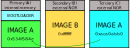
\includegraphics[width=1.1\textwidth, center]{figs/13}
  \par\end{center}
  \begin{itemize}
    \item image z C se překopíruje do A se standardním magic
    \item B necháme být, poslouží jako příští update slot
  \end{itemize}
\end{frame}

\begin{frame}[fragile]{Vytvoření image}
  Python script k přidání hlavičky před image
  \begin{verbatim}
    python3 apps/boot/nxboot/tools/nximage.py \
      --version VERSION \
      --header_size CONFIG_NXBOOT_HEADER_SIZE \
      --identifier 0x0 \
      nuttx.bin image.nximg
  \end{verbatim}
  \begin{itemize}
    \item script spočítá CRC a přidá specifikované položky
    \item stejný image lze použít pro přímé nahrání přes programátor i pro update
    \item hlavičku by mohl přidat i ld script, ale problém s počítáním CRC32
  \end{itemize}
\end{frame}

\begin{frame}[fragile]{Příklad -- kompilace bootloaderu}
  Příklad pro SAMv71 Xult Evaluation Kit
  \begin{small}
  \begin{verbatim}
  git clone \
  https://github.com/michallenc/incubator-nuttx.git nuttx
  git clone \
  https://github.com/michallenc/incubator-nuttx-apps.git apps
  cd nuttx
  git switch installfest2025
  ./tools/refresh.sh --silent samv71-xult:nxboot-loader
  mmake
  \end{verbatim}
  \end{small}
  Bootloader je nahrán na začátek programové paměti (třeba přes OpenOCD)
\end{frame}

\begin{frame}[fragile]{Příklad -- kompilace image}
  \begin{small}
  \begin{verbatim}
  make distclean
  ./tools/refresh.sh --silent samv71-xult:nxboot-updater
  mmake
  python3 ../apps/boot/nxboot/tools/nximage.py \
    --version "0.1.0" --header_size=0x200 -v \
    nuttx.bin nuttx.nximg
  \end{verbatim}
  \end{small}
  Image je nahrán do programové paměti za bootloader (třeba přes OpenOCD)
\end{frame}

\begin{frame}[fragile]{Příklad -- nahrání}
  Postup stejný jako u kompilace hlavního image a posuneme verzi.
  \begin{small}
  \begin{verbatim}
  python3 ../apps/boot/nxboot/tools/nximage.py \
    --version "0.2.0" --header_size=0x200 -v \
    nuttx.bin nuttx.nximg
  \end{verbatim}
  \end{small}
  K nahrání je možno použít program v desce (přístup přes konzoli).
  \begin{small}
    \begin{verbatim}
      nsh> nxboot_updater
    \end{verbatim}
  \end{small}
  Z počítače jde image poslat přes TCP jednoduchým scriptem
  \begin{small}
    \begin{verbatim}
      python3 ../apps/examples/nxboot-updater/sender.py \
        --host="ip adresa"
    \end{verbatim}
  \end{small}
  Update vyvolán restartem desky. Potvrzení pak z NuttX konzole.
  \begin{small}
    \begin{verbatim}
      nsh> nxboot_confirm
    \end{verbatim}
  \end{small}
  Další restart před potvrzením by vedl na revert.
\end{frame}

\begin{frame}{Závěrem}
  \begin{itemize}
    \item \smiley NuttX bootloader umožní spolehlivé a rychlé aktualizace se zálohou
    \item \smiley algoritmus šetrný k paměti
    \item \smiley nahrání lze provést pomocí téměř libovolného nástroje
    \item \smiley integrovaný v mainline NuttXu
    \item \frownie chybí šifrování
    \item \frownie sloty zabírají více místa v paměti
  \end{itemize}
\end{frame}

\begin{frame}{Odkazy}
  \begin{itemize}
    \item NuttX RTOS \url{https://nuttx.apache.org/}
    \item Updater Štěpána Pressla přes Silicon Heaven protokol
    \begin{itemize}
      \item \url{https://gitlab.fel.cvut.cz/otrees/motion/samocon}
      \item \url{https://silicon-heaven.github.io/shv-doc/}
    \end{itemize}
    \item Stránky OTREES s přednáškami k NuttXu a dalším tématům
    \begin{itemize}
      \item \url{https://gitlab.fel.cvut.cz/otrees/org/-/wikis/knowbase}
    \end{itemize}
  \end{itemize}
\end{frame}

\end{document}
